\section{Results and Discussion}
\label{sec:results}

\begin{figure*}[!t]
\centering
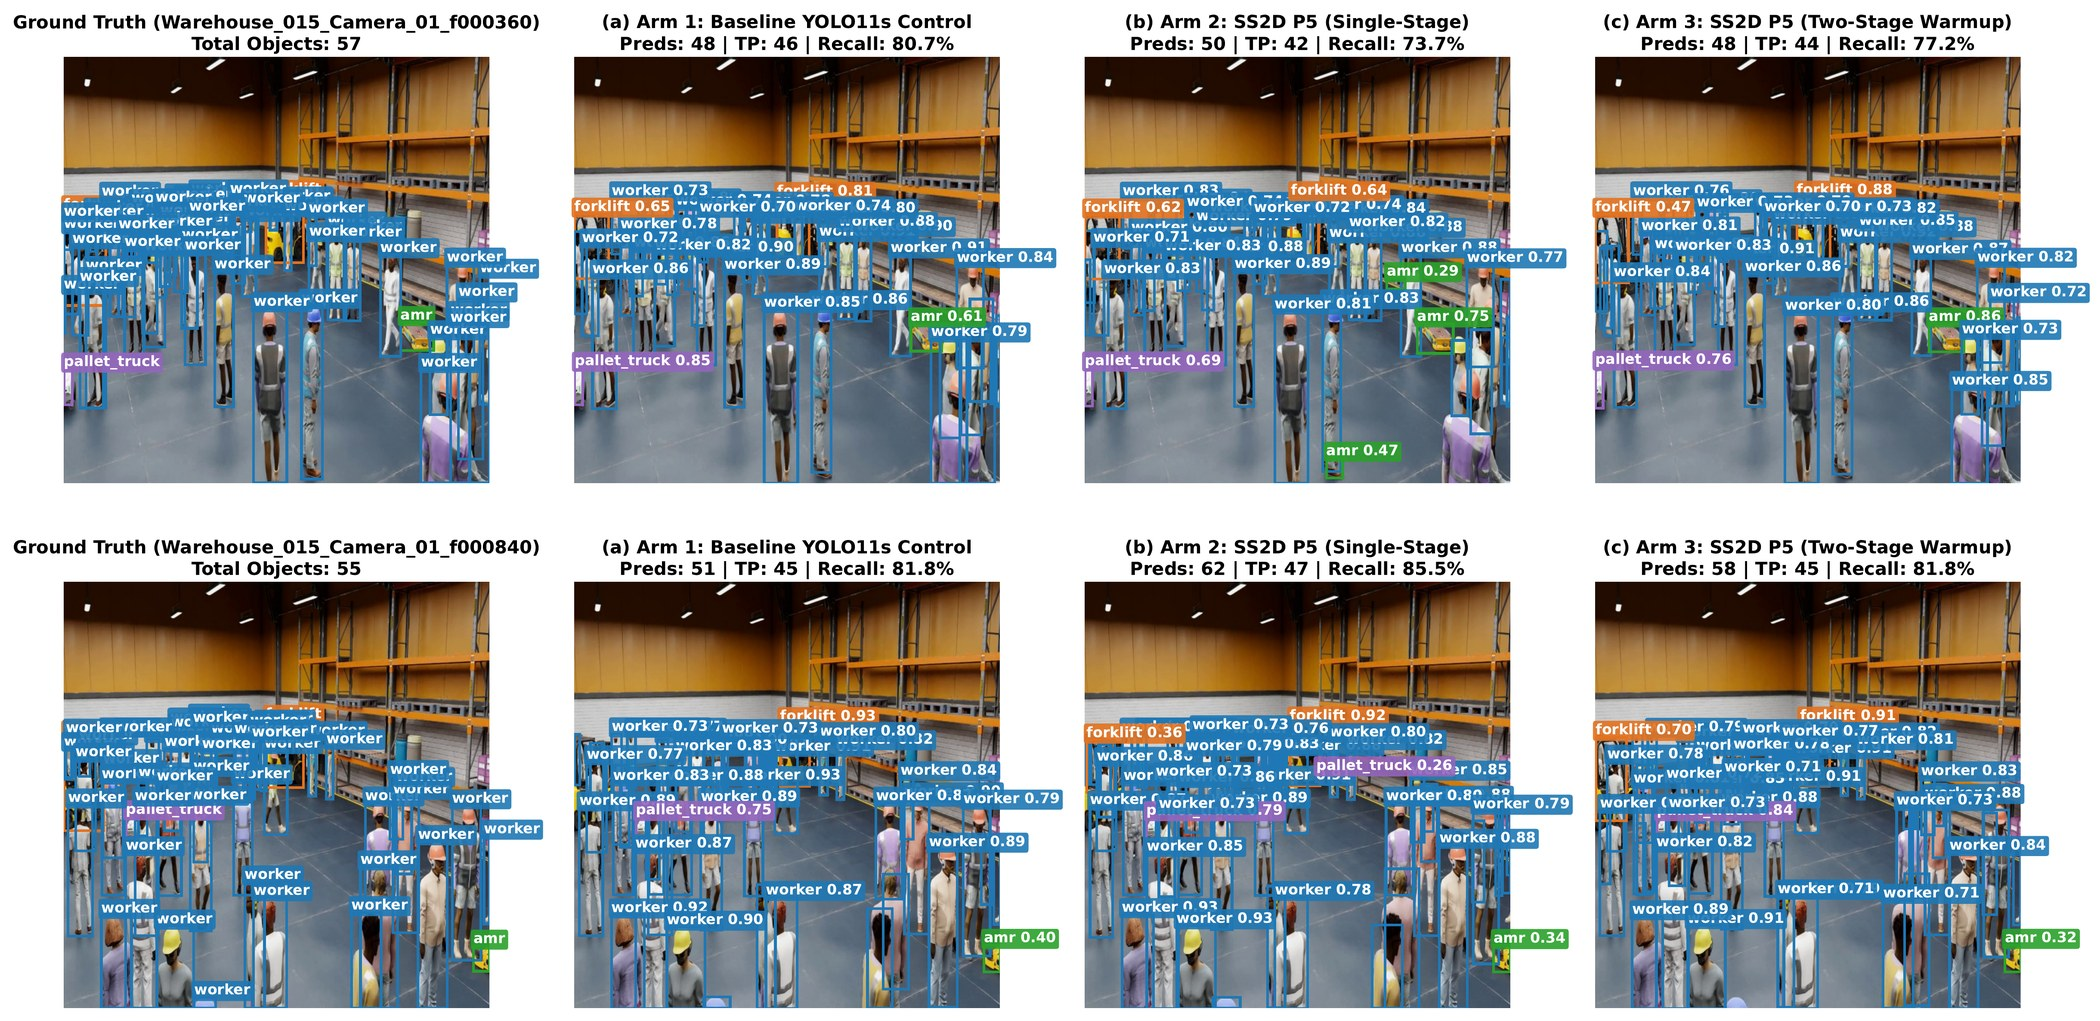
\includegraphics[width=0.98\textwidth]{figures/fig_qualitative_comparison.jpg}
\caption{Qualitative comparison on two SmartSpaces validation frames (Warehouse\_015, \texttt{Camera\_01}; the partition also used for checkpoint selection). Columns: ground truth; Arm 1 (baseline YOLO11s); Arm 2 (SS2D, single-stage); Arm 3 (SS2D, two-stage). Subtitles report the number of predictions, true positives (TP at $\text{IoU}\ge 0.5$), and recall ($\text{TP}/\text{GT}$).}
% TODO(authors): state how the two frames were chosen. JPEG made from the former PDF at 300 dpi (8.4 MB -> 0.6 MB).
\label{fig:qualitative_comparison}
\end{figure*}

\subsection{Architectural Footprint}
\label{sec:res_main}
Table~\ref{tab:main_results} compares the static footprint of the baseline and the Case B model.

\begin{table}[!t]
\caption{Architectural Footprint of the Baseline and the Case B Model}
\label{tab:main_results}
\centering
\footnotesize
\setlength{\tabcolsep}{3pt}
\begin{tabular}{lccccc}
\toprule
\textbf{Model} & \textbf{Layers} & \textbf{Params} & \textbf{GFLOPs} & \textbf{Weights} & \textbf{Host Lat.}$^{\ast}$ \\
 & & \textbf{(M)} & & \textbf{(MB)} & \textbf{(ms)} \\
\midrule
YOLO11s & 100 & 9.429 & 21.7 & 19.18 & 229.0 \\
SS2D (Case B)$^{\dagger}$ & 98 & 8.796 & 21.2 & 17.89 & 301.3 \\
\midrule
\textit{Change} & $-2$ & $-6.72\%$ & $-2.30\%$ & $-6.73\%$ & $+31.6\%$ \\
\bottomrule
\multicolumn{6}{p{0.95\columnwidth}}{\scriptsize $^{\ast}$Median forward latency, x86 host (Table~\ref{tab:edge_runtime}). $^{\dagger}$The checkpoint behind the x86 Case B file could not be confirmed; parameters, GFLOPs, and weights refer to the Arm~2 checkpoint.}
\end{tabular}
\end{table}

The Case B model has $6.72\%$ fewer parameters ($633{,}344$ fewer) and $21.2$ instead of $21.7$ GFLOPs; within Layer 10, the \texttt{WarehouseSS2DBlock} has $357{,}632$ parameters versus $990{,}976$ for \texttt{C2PSA} ($-63.9\%$; Table~\ref{tab:layer10_breakdown}). The checkpoint shrinks from $19.18$ to $17.89$\,MB. These static savings do not carry over to deployment: the exported ONNX file is larger ($38.5$ vs.\ $36.2$\,MiB) and runtime memory is higher (Section~\ref{sec:res_edge_deployment}).
% The former footprint bar chart (fig_architectural_comparison) was removed: it repeated Table V.

\subsection{Detection Accuracy and Convergence}
\label{sec:res_detection}
Table~\ref{tab:accuracy_results} summarizes accuracy after identical 20-epoch budgets.

% Auto-generated by scripts/make_tables.py - DO NOT EDIT MANUALLY
\begin{table}[!t]
\caption{Multi-Arm Convergence and Validated Checkpoint Study on SmartSpaces Warehouse}
\label{tab:accuracy_results}
\centering
\small
\resizebox{\columnwidth}{!}{%
\setlength{\tabcolsep}{3pt}
\begin{tabular}{lcccccc}
\toprule
\textbf{Experimental Arm} & \textbf{Final Ep. $\text{mAP}_{50}$} & \textbf{Peak Checkpoint $\text{mAP}_{50}$} & \textbf{Peak $\text{mAP}_{50-95}$} & \textbf{Precision} & \textbf{Recall} & \textbf{Val Box Loss} \\
\midrule
Arm 1: Baseline YOLO11s Control & 69.75\% & 69.75\% & 45.82\% & 0.818 & 0.572 & - \\
Arm 2: YOLO11s-SS2D (Case B, Single-Stage) & 65.46\% & 65.46\% & 41.56\% & 0.738 & 0.557 & - \\
Arm 3: YOLO11s-SS2D (Case B, Two-Stage Warmup) & 67.10\% & 67.10\% & 43.17\% & 0.725 & 0.645 & - \\
Arm 4: YOLO11s-SS2D (Case C, Dual-Scale P4+P5) & 67.17\% & 67.17\% & 42.73\% & 0.738 & 0.516 & - \\
\bottomrule
\end{tabular}%
}
\end{table}


Two views of the same runs must be distinguished (Table~\ref{tab:accuracy_results}, Fig.~\ref{fig:convergence_map}):
\begin{itemize}
    \item \textbf{Final epoch:} The baseline finishes at $69.75\%\ \text{mAP}_{50}$, ahead of Arm 4 ($67.17\%$), Arm 3 ($67.10\%$), and Arm 2 ($65.46\%$).
    \item \textbf{Best-fitness checkpoint:} Arm 2 reaches $71.95\%\ \text{mAP}_{50}$ (epoch 18) versus $69.80\%$ for the baseline (epoch 20), while Arm 3 reaches $67.67\%$ (stage-2 epoch 14) and Arm 4 $67.17\%$ (epoch 20).
\end{itemize}
The best-fitness checkpoint is selected on the same $100$-frame partition on which it is reported, so the $71.95\%$ figure is optimistically biased; at the final epoch the baseline leads all SS2D arms, and all SS2D arms have lower $\text{mAP}_{50-95}$ under either view. Validation $\text{mAP}_{50}$ also changes by up to $14$ points between consecutive epochs after epoch $5$, and by up to $33$ points in the first epochs of Arm 4 (Fig.~\ref{fig:convergence_map}), which exceeds the $+2.15$-point gap between Arm 2 and the baseline. One possible contributor is the change of training distribution when mosaic augmentation is switched off at epoch $11$ (Section~\ref{sec:exp_preprocessing}); we have not isolated this effect. With a single seed, the differences between arms cannot be distinguished from run-to-run variance.

\begin{figure}[!t]
\centering
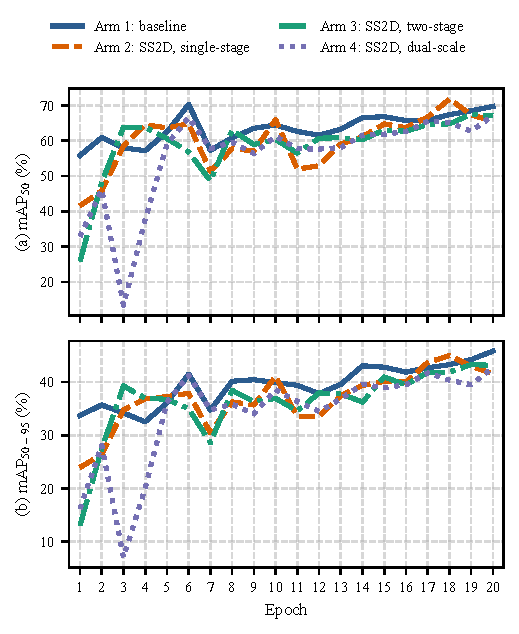
\includegraphics[width=\columnwidth]{figures/fig_convergence_map.pdf}
\caption{Validation accuracy over 20 epochs: (a) $\text{mAP}_{50}$ (\%); (b) $\text{mAP}_{50-95}$ (\%), for the baseline and the single-stage, two-stage, and dual-scale SS2D arms. For Arm 3, epochs 1--5 are stage 1 (frozen backbone) and epochs 6--20 are stage-2 epochs 1--15, so its best-fitness checkpoint (stage-2 epoch 14, Table~\ref{tab:accuracy_results}) appears at epoch 19.}
\label{fig:convergence_map}
\end{figure}

\subsection{Training Observations}
\label{sec:res_discussion}

\subsubsection{Transfer of Pretrained Head Weights}
In an initial version of the SS2D pipeline, adapting the COCO detection head ($80 \to 4$ classes) re-initialized not only the classification branch (\texttt{cv3}), which is required, but also the $42$ class-agnostic box-regression tensors (\texttt{cv2}) and the DFL parameters, raising the initial box loss to $\mathcal{L}_{\text{box}} = 6.276$. The baseline is not affected, because Ultralytics transfers all shape-compatible tensors when fine-tuning from \texttt{yolo11s.pt}. Transferring all shape-compatible tensors for the SS2D arms as well (the $42$ box-regression tensors and $336$ backbone and neck tensors) lowers the initial box loss to $2.758$. We regard this as a correction required for a fair comparison, not as a methodological contribution. The warmstart checkpoints and all SS2D models in Tables~\ref{tab:accuracy_results}--\ref{tab:edge_runtime} were produced with the earlier initialization, in which the output convolution was zero-initialized ($\mathbf{W}_{\text{out}} = \mathbf{0}$) ahead of a standard batch normalization; the zero-$\gamma$ initialization of Section~\ref{sec:mamba_integration} has not yet been re-evaluated end-to-end (Section~\ref{sec:limitations}).

\subsubsection{Single-Scale vs.\ Dual-Scale and Two-Stage Training}
Two-stage training (Arm 3) has the highest recall ($0.651$ vs.\ $0.572$ for the baseline, $+7.9$ percentage points) but also lower precision ($0.741$ vs.\ $0.818$, $-7.7$ points). Because Ultralytics reports both at the confidence threshold that maximizes F1, this is largely a shift of the operating point rather than a uniform improvement: the F1 score derived from these values is $0.693$ vs.\ $0.673$, and at the final epoch, where the baseline has precision $0.818$ and recall $0.572$ and Arm 3 has $0.725$ and $0.645$, it is $0.683$ vs.\ $0.673$. The dual-scale model (Arm 4) reaches $67.17\%\ \text{mAP}_{50}$ and $42.76\%\ \text{mAP}_{50-95}$, close to Arm 3, so adding a $P_4$ block brings no measurable accuracy benefit here, at a substantial runtime cost (Section~\ref{sec:res_edge_deployment}). All SS2D arms remain below the baseline in $\text{mAP}_{50-95}$ ($42.76$--$45.15\%$ vs.\ $45.53\%$).

\subsubsection{Per-Class Results}
Table~\ref{tab:per_class_results} reports per-class accuracy on the validation partition (also used for checkpoint selection).

% Auto-generated by scripts/make_tables.py - DO NOT EDIT MANUALLY
\begin{table}[!t]
\caption{Per-Class Detection Performance on Held-out Cross-Facility Validation Partition}
\label{tab:per_class_results}
\centering
\small
\resizebox{\columnwidth}{!}{%
\setlength{\tabcolsep}{3pt}
\begin{tabular}{lcccccccc}
\toprule
\textbf{Target Category} & \multicolumn{2}{c}{\textbf{Arm 1: Baseline}} & \multicolumn{2}{c}{\textbf{Arm 2: Single-Stage}} & \multicolumn{2}{c}{\textbf{Arm 3: Two-Stage}} & \multicolumn{2}{c}{\textbf{Arm 4: Dual-Scale}} \\\\
\cmidrule(lr){2-3} \cmidrule(lr){4-5} \cmidrule(lr){6-7} \cmidrule(lr){8-9}
& $\text{mAP}_{50}$ & $\text{mAP}_{50-95}$ & $\text{mAP}_{50}$ & $\text{mAP}_{50-95}$ & $\text{mAP}_{50}$ & $\text{mAP}_{50-95}$ & $\text{mAP}_{50}$ & $\text{mAP}_{50-95}$ \\\\
\midrule
\texttt{worker} (Personnel, $n=3{,}488$) & 89.2 & \textbf{63.2} & \textbf{89.3} & 61.9 & 87.9 & 60.5 & 88.5 & 60.9 \\
\texttt{forklift} (Heavy Machinery, $n=150$) & 70.1 & 31.8 & \textbf{79.7} & 38.3 & 76.3 & \textbf{38.4} & 75.2 & 33.8 \\
\texttt{pallet\_truck}$^{\dagger}$ (Manual Jack, $n=13$) & 32.8 & \textbf{22.4} & \textbf{33.9} & 17.7 & 22.9 & 16.2 & 20.0 & 14.6 \\
\texttt{amr} (Mobile Robot, $n=45$) & \textbf{87.1} & \textbf{64.7} & 84.9 & 62.6 & 83.7 & 57.5 & 85.0 & 61.7 \\
\midrule
\textbf{3-Class Macro (excl. pallet)} & 82.13 & \textbf{53.24} & \textbf{84.64} & 54.29 & 82.61 & 52.13 & 82.91 & 52.15 \\
\textbf{4-Class Global Macro (Peak)} & 69.80 & \textbf{45.82} & \textbf{71.95} & 41.56 & 67.67 & 43.17 & 67.17 & 42.73 \\
\textbf{4-Class Global Macro (Final Ep)} & \textbf{69.75} & - & 65.46 & - & 67.10 & - & 67.17 & - \\
\bottomrule
\multicolumn{9}{l}{\footnotesize $^{\dagger}$Notice on rare tail class: \texttt{pallet\_truck} contains only 13 validation instances ($0.35\%$ of total labels), exhibiting high sample variance.} \\\\
\end{tabular}%
}
\end{table}


\begin{enumerate}
    \item \textbf{Forklift:} All SS2D arms score above the baseline ($70.1\%$) on the $150$ forklift instances: Arm 2 $79.7\%$, Arm 3 $76.3\%$, Arm 4 $75.3\%\ \text{mAP}_{50}$. This is the largest and most consistent per-class difference. Because the instances come from $100$ sampled frames of two cameras, the number of distinct forklifts is much smaller than $150$, and the difference has not been tested across seeds or with a frame- or track-level bootstrap. The difference is an unisolated architectural effect: without trained identity or convolution-only replacements (Table~\ref{tab:g1_intervention} measures them for runtime only), it cannot be attributed to the selective scan rather than to the removal of \texttt{C2PSA} (for example, through reduced overfitting on $300$ training frames) or to run-to-run variance.
    \item \textbf{Worker:} The dominant class ($3{,}488$ of $3{,}696$ instances) changes little in $\text{mAP}_{50}$ ($87.9$--$89.4\%$), while all SS2D arms are lower in $\text{mAP}_{50-95}$ ($60.5$--$61.9\%$ vs.\ $63.2\%$).
    \item \textbf{AMR:} All SS2D arms are slightly below the baseline on the $45$ AMR instances ($83.7$--$85.0\%$ vs.\ $87.1\%\ \text{mAP}_{50}$).
    \item \textbf{Pallet truck:} All models score low ($20.0$--$33.9\%\ \text{mAP}_{50}$). With only $13$ validation instances ($0.35\%$ of labels), missing one or two objects shifts the AP substantially, so we do not interpret differences on this class. For reference, Table~\ref{tab:per_class_results} also lists a supplementary average over the three remaining classes; it was defined after inspecting the results, so we report it descriptively only. On these classes the SS2D arms are $0.5$ to $2.5$ points above the baseline in $\text{mAP}_{50}$, while in $\text{mAP}_{50-95}$ Arms 3 and 4 remain about $1$ point below it and Arm 2 is about $1$ point above it.
\end{enumerate}

\subsubsection{Qualitative Comparison}
Fig.~\ref{fig:qualitative_comparison} shows predictions on two dense validation frames. The picture is mixed: on frame \texttt{f000360} the baseline attains the highest recall ($80.7\%$ vs.\ $73.7\%$ for Arm 2 and $77.2\%$ for Arm 3), while on frame \texttt{f000840} Arm 2 is highest ($85.5\%$ vs.\ $81.8\%$ for both the baseline and Arm 3). On \texttt{f000360} the baseline also produces the fewest false positives ($2$ of $48$ predictions, vs.\ $8$ of $50$ for Arm 2 and $4$ of $48$ for Arm 3), consistent with its higher overall precision. These frames are illustrative only.

\subsection{Edge Deployment}
\label{sec:res_edge_deployment}
Table~\ref{tab:edge_runtime} reports ONNX Runtime measurements on the x86 host and on a Raspberry Pi~4 Model B Rev 1.2 (Broadcom BCM2711, quad-core Cortex-A72 at 1.5\,GHz, aarch64), using the protocol of Section~\ref{sec:exp_export}. Because the selective scan is written in standard PyTorch operators, the model exports to ONNX and runs on both devices without custom plugins.

\begin{table*}[!t]
\caption{ONNX Runtime Forward-Pass Latency and Memory ($640 \times 640$, Batch Size 1, FP32, CPU Execution Provider). Calls: Timed Calls; FPS $= 1000/\text{median}$; Rel.\ $=$ Median Relative to the Baseline on the Same Device, Session, and Thread Count. Memory: Peak RSS (High-Water Mark) on the Pi~4, RSS after the Timed Loop on the x86 Host.}
\label{tab:edge_runtime}
\centering
\footnotesize
\setlength{\tabcolsep}{4pt}
\begin{tabular}{llcccccc}
\toprule
\textbf{Model} & \textbf{Device (threads)} & \textbf{Calls} & \textbf{Memory (MiB)} & \textbf{Median (ms)} & \textbf{Mean $\pm$ SD (ms)} & \textbf{Rel.} & \textbf{FPS} \\
\midrule
YOLO11s (baseline) & x86 host (default) & 100 & 285.1 & 228.95 & 244.72 $\pm$ 33.5 & 1.00 & 4.37 \\
YOLO11s-SS2D (Case B, $P_5$)$^{\dagger}$ & x86 host (default) & 100 & 395.7 & 301.26 & 304.01 $\pm$ 8.5 & 1.32 & 3.32 \\
YOLO11s-SS2D (Case C, $P_4{+}P_5$) & x86 host (default) & 100 & 401.3 & 699.33 & 694.58 $\pm$ 12.1 & 3.05 & 1.43 \\
\midrule
\multicolumn{8}{l}{\textit{Raspberry Pi~4, session~2: baseline and Case B (trained Arm~3 export)}} \\
YOLO11s (baseline) & Pi 4 (1) & 100 & 233.2 & 3192.88 & 3194.63 $\pm$ 5.0 & 1.00 & 0.31 \\
YOLO11s-SS2D (Case B, $P_5$) & Pi 4 (1) & 100 & 373.1 & 3374.10 & 3374.58 $\pm$ 3.6 & 1.06 & 0.30 \\
YOLO11s (baseline) & Pi 4 (4) & 30 & 233.4 & 1117.27 & 1120.62 $\pm$ 7.5 & 1.00 & 0.90 \\
YOLO11s-SS2D (Case B, $P_5$) & Pi 4 (4) & 30 & 373.6 & 1314.26 & 1316.11 $\pm$ 4.8 & 1.18 & 0.76 \\
\midrule
\multicolumn{8}{l}{\textit{Raspberry Pi~4, session~1: baseline and Case C}} \\
YOLO11s (baseline) & Pi 4 (1) & 100 & 233.2 & 3360.50 & 3360.15 $\pm$ 5.2 & 1.00 & 0.30 \\
YOLO11s-SS2D (Case C, $P_4{+}P_5$) & Pi 4 (1) & 100 & 716.5 & 4178.68 & 4178.96 $\pm$ 3.5 & 1.24 & 0.24 \\
YOLO11s (baseline) & Pi 4 (4) & 30 & 233.3 & 1106.76 & 1110.09 $\pm$ 7.3 & 1.00 & 0.90 \\
YOLO11s-SS2D (Case C, $P_4{+}P_5$) & Pi 4 (4) & 30 & 718.3 & 1927.71 & 1929.04 $\pm$ 7.7 & 1.74 & 0.52 \\
\bottomrule
\multicolumn{8}{p{0.96\textwidth}}{\scriptsize $^{\dagger}$The checkpoint behind the x86 Case B file could not be confirmed (Section~\ref{sec:exp_export}). The single-thread baseline median differs by $5.0\%$ between the two Pi sessions (the clock of the session-1 single-thread runs was not logged), and the four-thread median by $0.9\%$; we therefore compare each model only with the baseline of its own session.} \\
\end{tabular}
\end{table*}

On the Pi, the peak memory of the Case B process is $373.6$\,MiB, $63.5\%$ below a $1$\,GiB budget; Case C peaks at $718.3$\,MiB and the baseline at $233.3$--$233.4$\,MiB. These peaks include session creation and agree with the RSS read after the timed loop to within $0.1$\,MiB. With four threads, forward-pass throughput on the Cortex-A72 is $0.76$\,FPS for Case B and $0.52$\,FPS for Case C, versus $0.90$\,FPS for the baseline. These rates are far from real-time ($\geq 30$\,FPS) and exclude preprocessing and NMS; the CPU results therefore establish operator portability and that the models fit a $1$\,GiB memory budget, not real-time capability.

\subsubsection{Why the Cheaper Model Is Slower}
Despite fewer parameters ($8.796$ vs.\ $9.429$\,M) and FLOPs ($21.2$ vs.\ $21.7$ GFLOPs), Case B is slower than the baseline in every setting: by $31.6\%$ in median on x86, and on the Cortex-A72 by $5.7\%$ with one thread ($3374.10$ vs.\ $3192.88$\,ms) and $17.6\%$ with four threads ($1314.26$ vs.\ $1117.27$\,ms). Table~\ref{tab:graph_profile} and the measurements suggest the following explanation.
\begin{enumerate}
    \item \textbf{Graph unrolling:} The baseline exports to $320$ ONNX nodes. Exporting the sequential four-direction scan unrolls its loop over $L = 400$ steps into $14{,}771$ nodes ($4{,}800$ \texttt{Gather}, $3{,}293$ \texttt{Mul}, $3{,}212$ \texttt{Unsqueeze}, $1{,}621$ \texttt{Add}, and $1{,}600$ \texttt{ReduceSum}); ONNX Runtime's graph optimizer removes only $70$ of them. Case C, which adds a scan over $L = 1{,}600$ tokens at $P_4$, has $90{,}201$ nodes ($72{,}385$ after optimization).
    \item \textbf{Time moves outside the convolutions:} Convolution kernel time per call is nearly the same in the three models ($905$, $865$, and $877$\,ms), but its share of kernel time falls from $78.4\%$ (baseline) to $50.0\%$ (Case B) and $22.5\%$ (Case C), while the small element-wise and indexing operators of the scan take $35.1\%$ and $68.4\%$. The profiler adds a per-node cost (mean profiled call $1161$, $1951$, and $4943$\,ms vs.\ the unprofiled medians above), so these shares overstate the scan's share, especially for Case C; the near-constant convolution time is the more robust observation. Together with the analytical result that the scan's arithmetic is small (Table~\ref{tab:mixing_cost}), this indicates that the extra latency comes from the many small operators executed per call rather than from arithmetic.
    \item \textbf{Poor multi-core scaling:} Going from one to four threads speeds up the baseline by $2.86\times$ but Case B by only $2.57\times$ (session~2), and the baseline by $3.04\times$ but Case C by only $2.17\times$ (session~1), so the gap to the baseline widens with the thread count ($1.06 \to 1.18$ for Case B, $1.24 \to 1.74$ for Case C). This is consistent with a long chain of small, dependent operators that leave little work to parallelize within each operator. Case B also uses $60.1\%$ more peak memory than the baseline ($373.6$ vs.\ $233.4$\,MiB), consistent with materializing intermediate tensors for each operator.
\end{enumerate}
These observations are correlational. Section~\ref{sec:res_intervention} therefore changes the graph form of the scan while keeping its computation fixed.

\begin{table}[!t]
\caption{ONNX Graph Size and Operator Profile on the Pi~4 (Four Threads, ONNX Runtime Profiler, Five Profiled Calls)}
\label{tab:graph_profile}
\centering
\footnotesize
\setlength{\tabcolsep}{2.5pt}
\begin{tabular}{lccccc}
\toprule
\textbf{Model} & \textbf{Nodes} & \textbf{ORT nodes} & \textbf{MiB} & \textbf{Conv ms} & \textbf{Conv/scan \%} \\
\midrule
Baseline & 320 & 236 & 36.2 & 905 & 78.4 / $<2.5$ \\
Case B & 14{,}771 & 14{,}701 & 38.5 & 865 & 50.0 / 35.1 \\
Case C & 90{,}201 & 72{,}385 & 46.6 & 877 & 22.5 / 68.4 \\
\bottomrule
\multicolumn{6}{p{0.95\columnwidth}}{\scriptsize ORT nodes: after ONNX Runtime graph optimization. MiB: ONNX file size. Conv ms: convolution kernel time per profiled call. Conv/scan \%: share of summed kernel time taken by convolutions and by the scan operators, i.e., \texttt{Mul}, \texttt{Squeeze}, \texttt{Unsqueeze}, \texttt{Add}, \texttt{ReduceSum}, \texttt{Gather}, and \texttt{Split}; for the baseline, only \texttt{Split} and \texttt{Add} ($2.0\%$) appear among its ten most expensive operator types, and each remaining type takes at most $0.1\%$. Baseline and Case C were profiled in session~1 without a clock log, Case B in session~2 at $1.5$\,GHz.}
\end{tabular}
\end{table}

\subsubsection{Runtime Intervention: Graph Form of the Scan}
\label{sec:res_intervention}
Table~\ref{tab:g1_intervention} reports the intervention of Section~\ref{sec:exp_export}. Three results stand out.
\begin{enumerate}
    \item \textbf{Removing attention saves little:} Removing the $P_5$ block entirely lowers latency by only $2.4\%$ (one thread) and $5.3\%$ (four threads), and the convolution-only block costs about the same as no block. The SS2D block, by contrast, adds $17.0\%$ and $22.2\%$ over the identity model, so its overhead is neither explained nor offset by the removal of \texttt{C2PSA}.
    \item \textbf{Fewer nodes did not mean lower latency:} One ONNX \texttt{Loop} per direction shrinks the graph from $14{,}767$ to $367$ nodes but makes the model $2.2\times$ (one thread) and $4.5\times$ (four threads) slower than the unrolled scan. The loop body has $37$--$38$ nodes and runs $400$ times per direction, so about $60{,}000$ node executions remain per call, more than in the unrolled graph. The chunked scan ($T = 4$) cuts the graph by $43\%$ but adds computation within each chunk and is $4.4\%$ and $14.0\%$ slower than the unrolled scan.
    \item \textbf{Implication:} Static node count is therefore not the cause of the overhead. The data are better explained by the cost of executing a long chain of small, dependent operations, whether unrolled or looped; we have not isolated the per-operator scheduling cost with hardware counters. None of the plugin-free forms we tried closed the gap; parallel associative scans~\cite{blelloch1990prefix, dao2024mamba2} remain untested.
\end{enumerate}
With untrained weights, the unrolled SS2D export runs within $0.2\%$ of the trained Case B export with four threads but $6.5\%$ slower with one thread, so the absolute values in Table~\ref{tab:g1_intervention} should not be compared with Table~\ref{tab:edge_runtime}.

\begin{table}[!t]
\caption{Runtime Intervention on the Pi~4 (Session~2, Untrained Exports, $3$ Warmup and $20$ Timed Calls). Rel.\ $=$ Median Relative to the Baseline at the Same Thread Count}
\label{tab:g1_intervention}
\centering
\footnotesize
\setlength{\tabcolsep}{2pt}
\begin{tabular}{lcccccc}
\toprule
\textbf{Variant} & \textbf{Nodes} & \textbf{1 thr.} & \textbf{Rel.} & \textbf{4 thr.} & \textbf{Rel.} & \textbf{MiB} \\
\midrule
Baseline (\texttt{C2PSA}) & 320 & 3146.7 & 1.00 & 1132.8 & 1.00 & 233.3 \\
$P_5$ block removed & 292 & 3070.4 & 0.98 & 1072.7 & 0.95 & 229.4 \\
Convolution-only & 300 & 3105.4 & 0.99 & 1095.9 & 0.97 & 230.5 \\
SS2D, unrolled & 14{,}767 & 3593.8 & 1.14 & 1311.3 & 1.16 & 373.6 \\
SS2D, ONNX \texttt{Loop} & 367 & 7778.6 & 2.47 & 5938.4 & 5.24 & 274.0 \\
SS2D, chunked ($T = 4$) & 8{,}355 & 3752.5 & 1.19 & 1494.7 & 1.32 & 304.3 \\
\bottomrule
\multicolumn{7}{p{0.95\columnwidth}}{\scriptsize Median latency in ms; standard deviations are at most $10.8$\,ms. MiB: peak RSS with four threads. The three SS2D rows compute the same function (Section~\ref{sec:exp_export}); the untrained unrolled export has four nodes fewer than the trained Case B export.} \\
\end{tabular}
\end{table}

\subsection{Design Lessons for Hybrid CNN--SSM Detectors on Edge CPUs}
\label{sec:lessons}
The measurements above point to three practical lessons for engineers who replace attention with selective scans in small detectors.
\begin{enumerate}
    \item \textbf{Fewer FLOPs can mean a slower model.} At $P_5$ ($L = 400$), attention is already cheap, and the replacement saves parameters mainly by narrowing channels (Table~\ref{tab:layer10_breakdown}). The sequential scan, however, is slower and uses more memory on CPU (Table~\ref{tab:edge_runtime}), and the gap widens with the thread count. Shrinking the graph did not help: an ONNX \texttt{Loop} or a chunked scan with far fewer nodes was slower still (Table~\ref{tab:g1_intervention}). FLOPs and node count are therefore both poor guides; latency and peak memory should be measured at the deployed thread count, and alternative export forms of the recurrence should be compared directly.
    \item \textbf{Comparisons need identical warm starts.} When a COCO head is adapted to a new class count, the class-agnostic box-regression branch must be kept for every arm; otherwise the modified model starts from a higher loss ($6.276$ vs.\ $2.758$) and the comparison is biased against it (Section~\ref{sec:res_discussion}).
    \item \textbf{A zero-initialized convolution ahead of batch normalization is not an identity initialization.} It holds only at step $0$; afterwards batch normalization rescales the branch to full scale (Eq.~\eqref{eq:zero_wout}). Zero-$\gamma$ initialization (Eq.~\eqref{eq:zero_gamma}) avoids this by construction; we propose it for future warm-start integration, although its effect on detector training remains to be measured.
\end{enumerate}

\subsection{Limitations}
\label{sec:limitations}
The results above should be read with the following limitations. (i) All accuracy results come from a single training seed, a 20-epoch budget, and a single $100$-frame validation facility that also served for checkpoint selection; no held-out test facility was evaluated and no significance testing was performed. (ii) The dataset is synthetic (NVIDIA Omniverse), covers two facilities, and consecutive sampled frames are highly correlated; transfer to real warehouses is untested. (iii) The \texttt{pallet\_truck} class has only $13$ validation instances, so its per-class results are not interpreted. (iv) The reported SS2D models were trained with a zero-initialized output convolution preceding batch normalization; the zero-$\gamma$ initialization of Section~\ref{sec:mamba_integration} has not yet been re-evaluated end-to-end. (v) Identity and convolution-only replacements were measured for runtime only (Table~\ref{tab:g1_intervention}), not trained, so no ablation separates the accuracy contribution of the selective scan from that of removing \texttt{C2PSA}, and the simplifications relative to standard Mamba blocks (Section~\ref{sec:mamba_integration}) are not ablated. (vi) Edge measurements cover only the forward pass on two CPUs with FP32 ONNX Runtime; preprocessing, NMS, session-creation time (which we observed to reach tens of minutes for Case C on the Pi but did not time), GPU/NPU accelerators, quantized models, and energy were not measured. Without active cooling, four-thread runs on the Pi were limited to $30$ timed calls to avoid thermal clock reduction, and x86 memory is reported after the timed loop rather than as a peak. (vii) The Pi results come from two sessions whose single-thread baseline medians differ by $5.0\%$; each model is compared only with its same-session baseline. An earlier Case B measurement used a pre-fine-tuning export by mistake and is superseded; the checkpoint behind the x86 Case B row could not be confirmed. The intervention uses untrained exports, whose absolute single-thread latency differed from the trained Case B export by $6.5\%$.
